This chapter provides essential background information and reviews relevant prior research. It commences with an introduction to the sub-task of Question Answering (\gls{qa}), as presented in Section \ref*{sec:qa}. As previously mentioned in the Introduction (Chapter \ref{chap:intro}), this chapter maintains a clear distinction between \gls{qa} and \gls{convqa}. Consequently, Section \ref{sec:cqa} extends upon the foundational knowledge of \gls*{qa} and introduces the requisite concepts for the transformation of a QA-System into a \gls{convqa}-System. Section \ref{sec:related_work} will delve into the related work, providing a comprehensive overview of the current state-of-the-art in the field of \gls{qa} and \gls{convqa} over textual knowledge sources.

\section{Question Answering}
\label{sec:qa}

The evolution of \gls{qa} as a research field provides a solid foundation for understanding current research initiatives and methodologies. Among the early contributions is BASEBALL, an automated \gls{qa} system developed by researchers at \gls{mit} in 1961. This QA system demonstrated its capability to answer questions related to baseball using natural English language \cite{green_baseball_1961}.


In 1999, \gls{trec} (Text Retrieval Conference) initiated the \gls{trec}-8 Question Answering track, which marked "the first large-scale evaluation of domain-independent question-answering systems" \cite{voorhees_trec-8_1999}. A more well-known QA system is \textit{Watson} by IBM, an open-domain \gls{qa} system that won a the TV show Jeopardy! in 2011 \cite{ferrucci_introduction_2012}. It is evident that an evolutionary process has occurred between the early research in 1961 and today's systems like \textit{ChatGPT} by OpenAI. To understand the dimensions in which these systems differ, their components, and how to distinguish them will be introduced in Section \ref{subsec:qa_basics}, while subsequent sections will delve deeper into specific components.

In 1999, the \gls{trec} initiated the \gls{trec}-8 Question Answering track, marking \enquote{the first large-scale evaluation of domain-independent question-answering systems} \cite{voorhees_trec-8_1999}. A more renowned QA system is IBM's \textit{Watson}, an open-domain \gls{qa} system that famously triumphed on the television game show Jeopardy! in 2011 \cite{ferrucci_introduction_2012}. It is evident that an evolutionary process has transpired between the early research in 1961 and contemporary systems such as OpenAI's \textit{ChatGPT}. In section \ref{subsec:qa_basics} we will lay the groundwork by introducing the fundamental aspects of \gls{qa}-Systems and the techniques used to differentiate and categorize them. Following that, subsequent sections will delve deeper into the examination of specific system components.


\subsection{Basics}
\label{subsec:qa_basics}

Jurafsky and Martin define a \gls{qa}-System as a system \enquote{designed to satisfy human information needs} \cite{jurafsky_speech_2023}. Hence, it primarily functions as an Information Retrieval System, with its primary objective being to provide users with the desired and accurate information in response to natural language requests.

The research community has yet to establish a universally accepted classification framework for Question Answering (QA) systems. For instance, Hao et al. and Farea et al. \cite{hao_recent_2022, farea_evaluation_2022} take a comprehensive approach to classify QA systems but differ in certain aspects, such as their treatment of question types and knowledge sources. On the other hand, other researchers \cite{zhu_retrieving_2021, jurafsky_speech_2023, etezadi_state_2023, zhang_survey_2023} employ a similar classification methodology but often focus solely on retrieval-based approaches, thereby lacking a holistic perspective.

The classification proposed by Farea et al. \cite{farea_evaluation_2022} goes a step further by distinguishing between the \textbf{QA-Framework} and \textbf{QA-Paradigms}, enhancing its versatility for comparing classical and modern QA systems. An adaptation of this classification will be utilized in this thesis. The originally proposed QA algorithms have been extended to include the Retrieval-based approach, and the Question Types have been revised based on the typology introduced by Mishra et al. in their 2016 survey \cite{mishra_survey_2016}, which was further elaborated upon by Etezadi et al. \cite{etezadi_state_2023}. In this context, a crucial distinction is made between a \textbf{QA} and \textbf{ConvQA} system, guided by the criteria outlined in \cite{zamani_conversational_2023}: a QA system exclusively handles standalone questions, while any inquiry exceeding a single question and involving conversational context falls within the domain of a \textbf{ConvQA} system.

The \textbf{\gls{qa}-Framework} encompasses external factors such as Question and Answer Types, while also considering system-related factors like the \gls{qa} Algorithm and Knowledge Source \cite{farea_evaluation_2022, hao_recent_2022}. Conversely, the \textbf{\gls{qa}-Paradigm} defines the fundamental underlying concept of a system and can be seen as a subset of possible combinations within the \textbf{\gls{qa} Framework}. Currently, three dominant paradigms prevail:

\begin{enumerate}
    \item \textbf{Information Retrieval (IR)-Based QA}: This paradigm involves searching through extensive multi-modal data based on a user's question and using the retrieved passages to generate an answer.
    
    \item \textbf{Knowledge Base (KB) QA}: In this approach, a semantic representation of the question is constructed, and a knowledge base is queried using this representation. The returned results are then used to generate an answer.
    
    \item \textbf{Generative Question Answering}: Here, knowledge is fully implicit, and a neural network (NN) generates answers based on its trained parameters.
\end{enumerate}

For visual clarity, a diagram illustrating the adjusted \gls{qa} Framework Classification by Farea et al. is provided in Figure \ref{fig:qa_classification}.

\begin{figure}
    \centering
    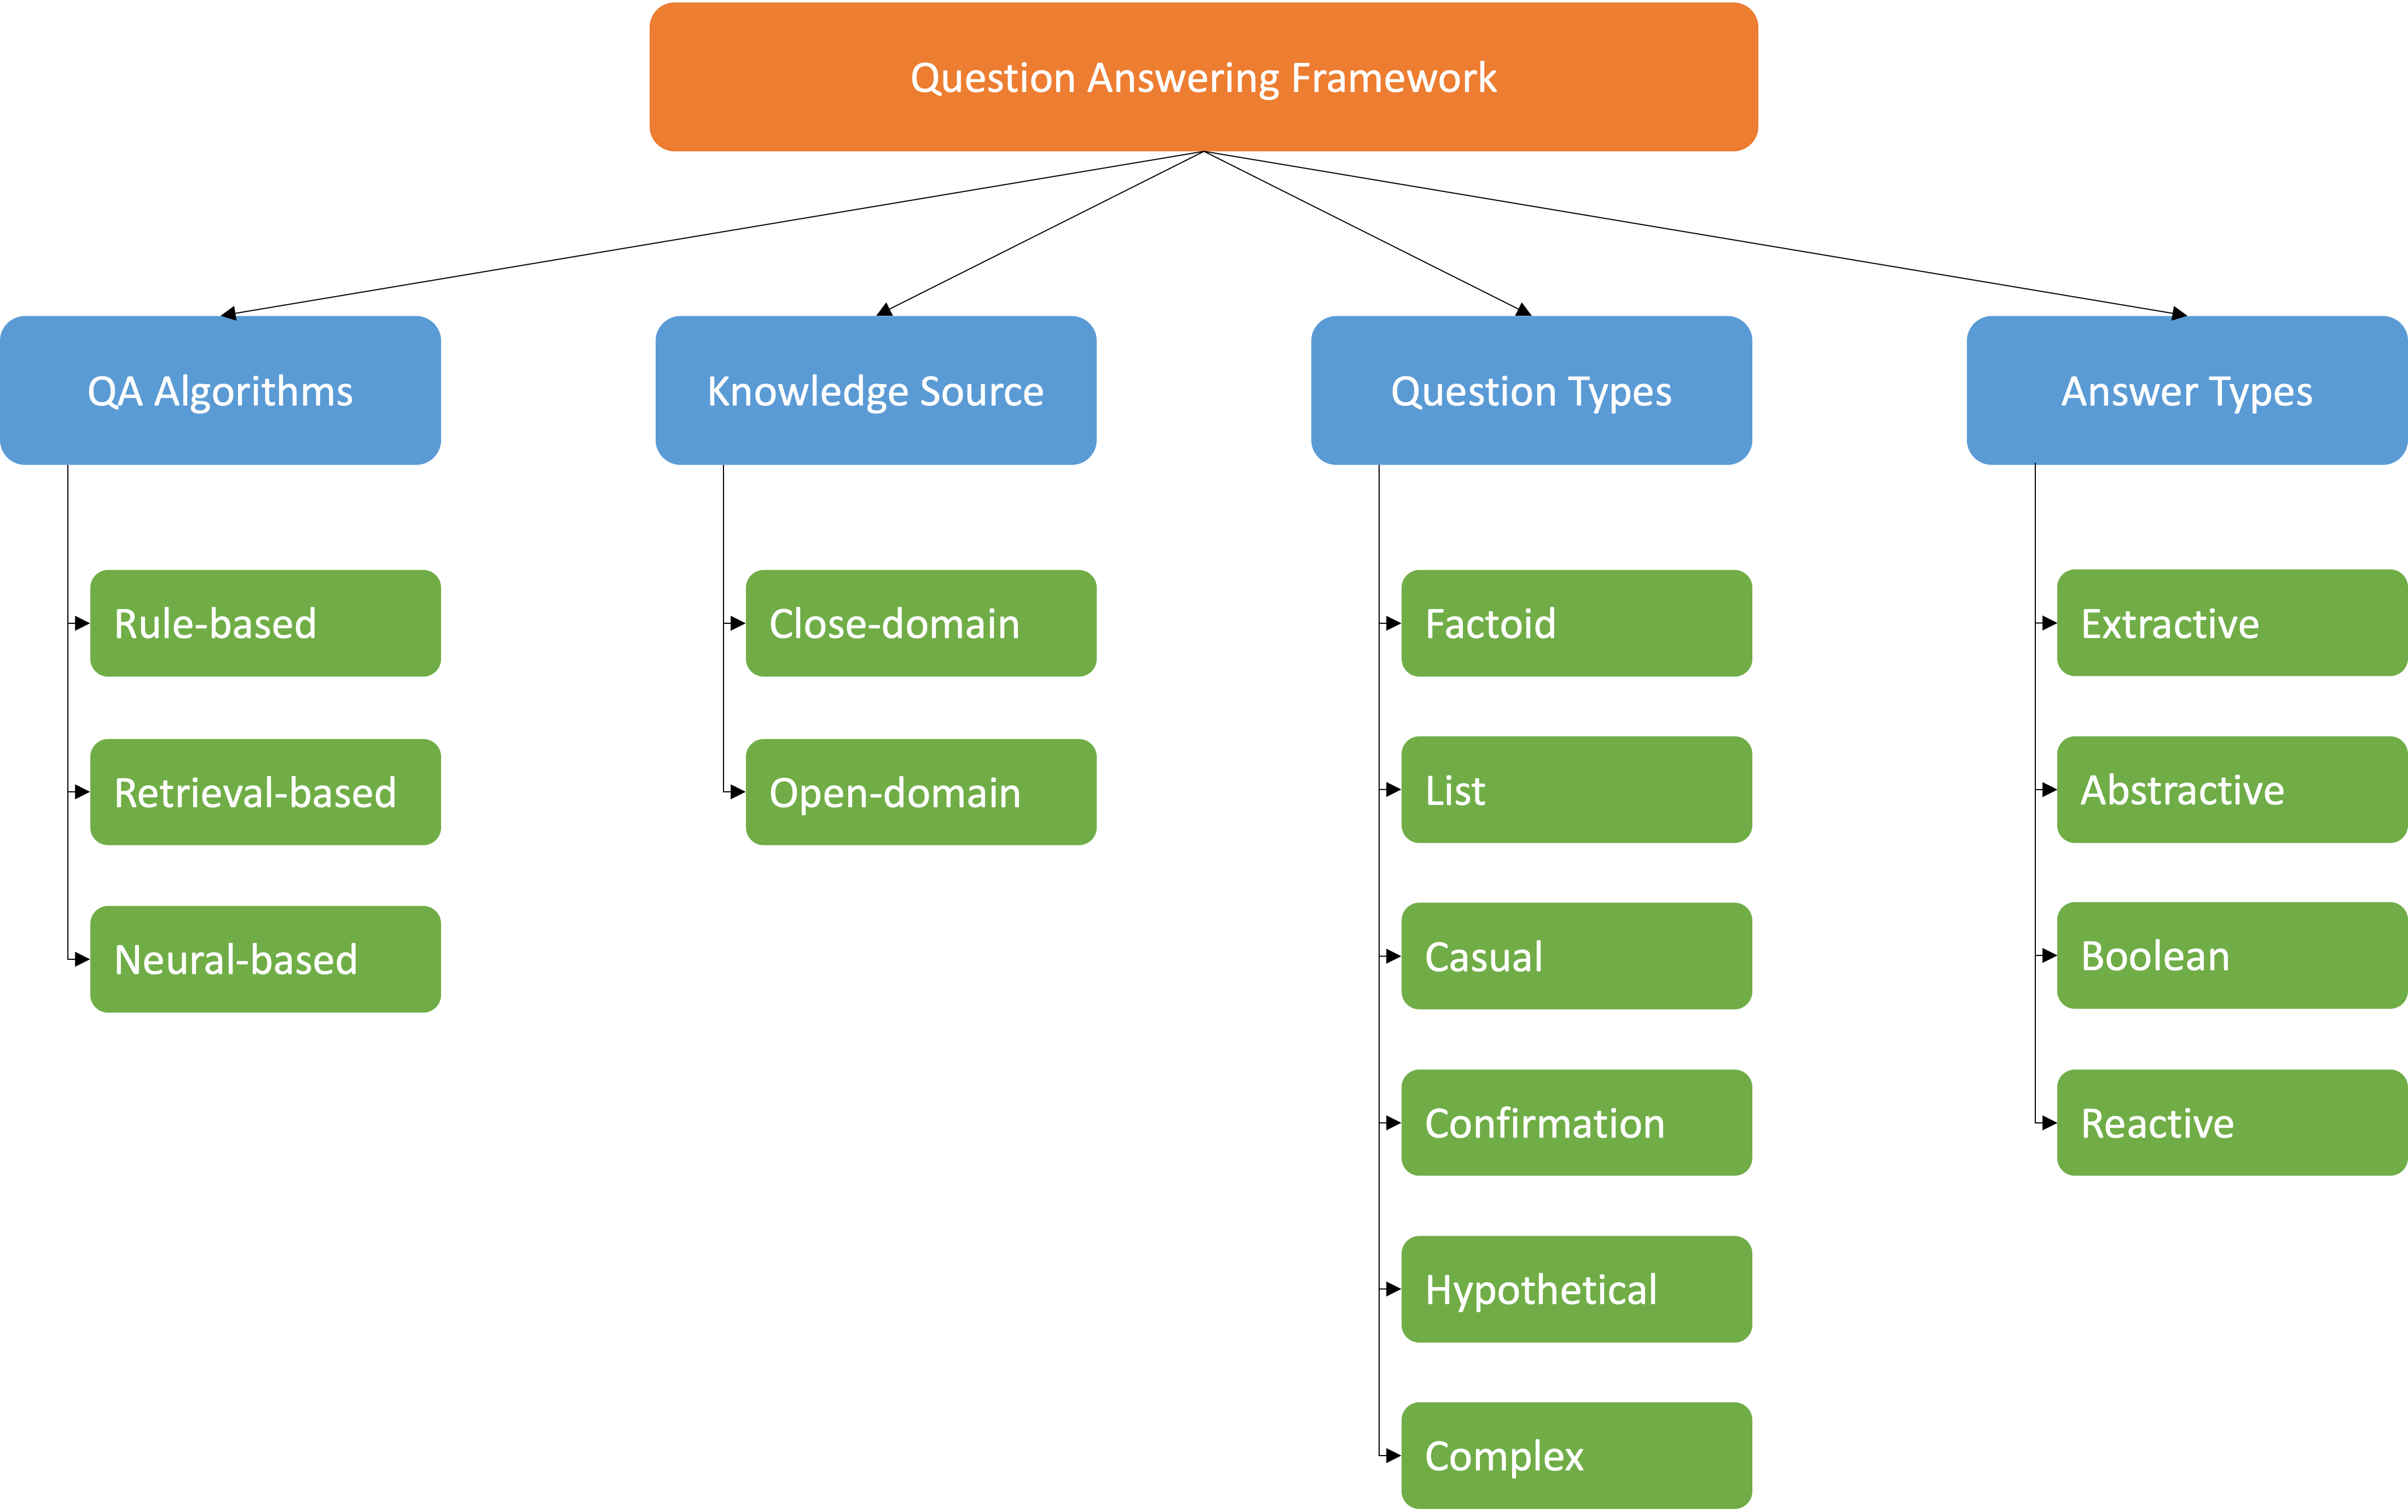
\includegraphics[width=\textwidth]{Grafiken/QA_Framework.png}
    \caption{Adjusted \gls{qa} Framework Classification by Farea et al. \cite{farea_evaluation_2022}}
    \label{fig:qa_classification}
\end{figure}


Figure \ref{fig:qa_classification} illustrates the aforementioned classification. The primary distinguishing factor is the employed \textbf{\gls{qa} Algorithm}. Rule-based approaches involve the manual crafting of feature extractions from user questions, which are then compared to the knowledge base. Rule-based approaches are typically employed in closed-domain \gls{qa} systems exclusively \cite{etezadi_state_2023}.

Retrieval-based approaches are the classic Information Retrieval (IR)-based \gls{qa} systems, comprising two key components: an intent classifier and a retriever. The intent classifier's objective is to discern the question's intent and identify important entities. Subsequently, the retriever searches the knowledge source and identifies the most relevant passages \cite{farea_evaluation_2022, zhu_retrieving_2021}.

The Neural-based approach, often referred to as the generative approach, utilizes a Sequence-to-Sequence (S2S) model to generate accurate answers to given questions. In this paradigm, the information is stored directly in the neural network's parameters, otherwise the neural network is part of a Retrieval-based approach. Most datasets in these contexts consist of triples of question, context, and answer pairs \cite{jurafsky_speech_2023}. Notably, widely used datasets such as SQuAD and QASPER originally emerged from the field of machine reading comprehension, representing a foundational step in the evolution of \gls{qa} systems \cite{rajpurkar_squad_2016, dasigi_dataset_2021, zhu_retrieving_2021}.

In addition to the \textbf{\gls{qa} Algorithms}, the \textbf{Knowledge Source} plays a pivotal role in distinguishing various aspects of Question Answering (QA) systems. The nature of the knowledge source can range from structured to unstructured or semi-structured, and it may encompass diverse data modalities, including text, audio, and video. A common point of comparison in the QA landscape is between closed and open-domain systems.

In the broad sense, a \textbf{closed-domain} QA system operates within the confines of a specific knowledge domain, which means it has limited access to information. In contrast, \textbf{open-domain} QA systems grapple with an extensive array of knowledge sources, necessitating a more versatile approach \cite{farea_evaluation_2022}.

Furthermore, a closed-domain setup often entails limitations on the types of questions it can handle, primarily focusing on factoid questions or predefined templates. Additionally, it frequently relies on structured knowledge bases like graphs or logically organized repositories \cite{hao_recent_2022}.

Conversely, open-domain QA systems are designed to tackle a wide spectrum of user queries, ranging from factoids to more complex inquiries. They typically deal with unstructured knowledge sources, which can be substantial and diverse in content \cite{zhu_retrieving_2021, farea_evaluation_2022, jurafsky_speech_2023}.

An alternative perspective for distinguishing \gls{qa}-Systems lies in the \textbf{Question Types} that users can input into the system. Questions can fall into various categories, such as \textit{factoid, list, casual, confirmation, hypothetical} \cite{mishra_survey_2016}, or \textit{complex} \cite{etezadi_state_2023}.

\begin{itemize}
   \item \textit{Factoid questions}, the most common type, are typically signaled by question words (what, when, which, who, how) and yield a concise factual answer.
   
   \item \textit{List questions} represent a specialized subset of factoid questions, where the answer comprises a list of facts.
   
   \item \textit{Casual questions} encompass inquiries that deviate from the factoid format, often involving words like \textit{how} or \textit{why} and requiring more advanced reasoning.
   
   \item \textit{Confirmation questions} seek simple yes or no responses, frequently employed in personal assistant applications.
   
   \item \textit{Hypothetical questions} delve into hypothetical scenarios (e.g., "what would happen if"), aiming for plausible rather than definitive answers.
   
   \item \textit{Complex questions} can be further categorized into \textit{answer-retrieval-complex} and \textit{question-understanding-complex}. In the case of question-understanding-complex questions, the complexity arises from nuances like multiple constraints, making the question itself intricate to comprehend. In contrast, answer-retrieval-complex questions involve complexities in finding the correct answer, often requiring the combination of information from multiple documents or similar sources. This is commonly referred to as long-form \gls{qa}.
\end{itemize}

Lastly, a \gls{qa}-System can be characterized by the \textbf{Answer Types} it offers, a concept closely intertwined with Question Types. Farea et al. \cite{farea_evaluation_2022} delineate three categories of answers: \textit{span, abstractive,} and \textit{agnostic}. 

\begin{itemize}
   \item \textit{Span answers} represent the most common type, where the answer is a specific factual excerpt presented as a span of tokens.
   
   \item \textit{Abstractive answers} often arise in response to confirmation questions and can be a system-generated reaction based on the user's provided answer.
   
   \item \textit{Agnostic answers} typically correspond to complex questions that necessitate the system to consider multiple documents and information sources to formulate a response. In such cases, no predefined or annotated answer exists.
\end{itemize}

% Pushed 1st

\subsection{Information Retrieval Architectures}
\label{subsec:qa_architectures}

As stated in the previous section (Section \ref{subsec:qa_basics}), there are three major paradigms in \gls{qa}: \gls{ir}-based \gls{qa}, \gls{kb}-based QA, and Generative \gls{qa}. This section will primarily concentrate on the first paradigm, \gls{ir}-based QA, as it holds the most promise for addressing the objectives of this thesis topic.

This thesis will not focus on \gls{kb} QA, as this approach requires the mapping of the query to a structured data representation. As the task of this thesis is to develop a general system, which is adaptable to different data inputs, \gls{kb} QA will be excluded \cite{dimitrakis_survey_2020}.

Generative \gls{qa} is often denoted as \textit{Retriever-free} or \textit{Neural-based} approaches. The central characteristic of this paradigm is that knowledge resides within the parameters of a neural network. Consequently, the knowledge is implicit, and the \gls{qa} system will not furnish a specific document, passage, or other source from which it extracted the information. Instead, it offers a textual excerpt. While these systems can achieve competitive performance compared to \gls{ir}-based \gls{qa} systems, they are not under consideration for this thesis due to their lack of reference, which is a crucial requirement for the system to be developed \cite{roberts_how_2020}.


\begin{figure}
    \centering
    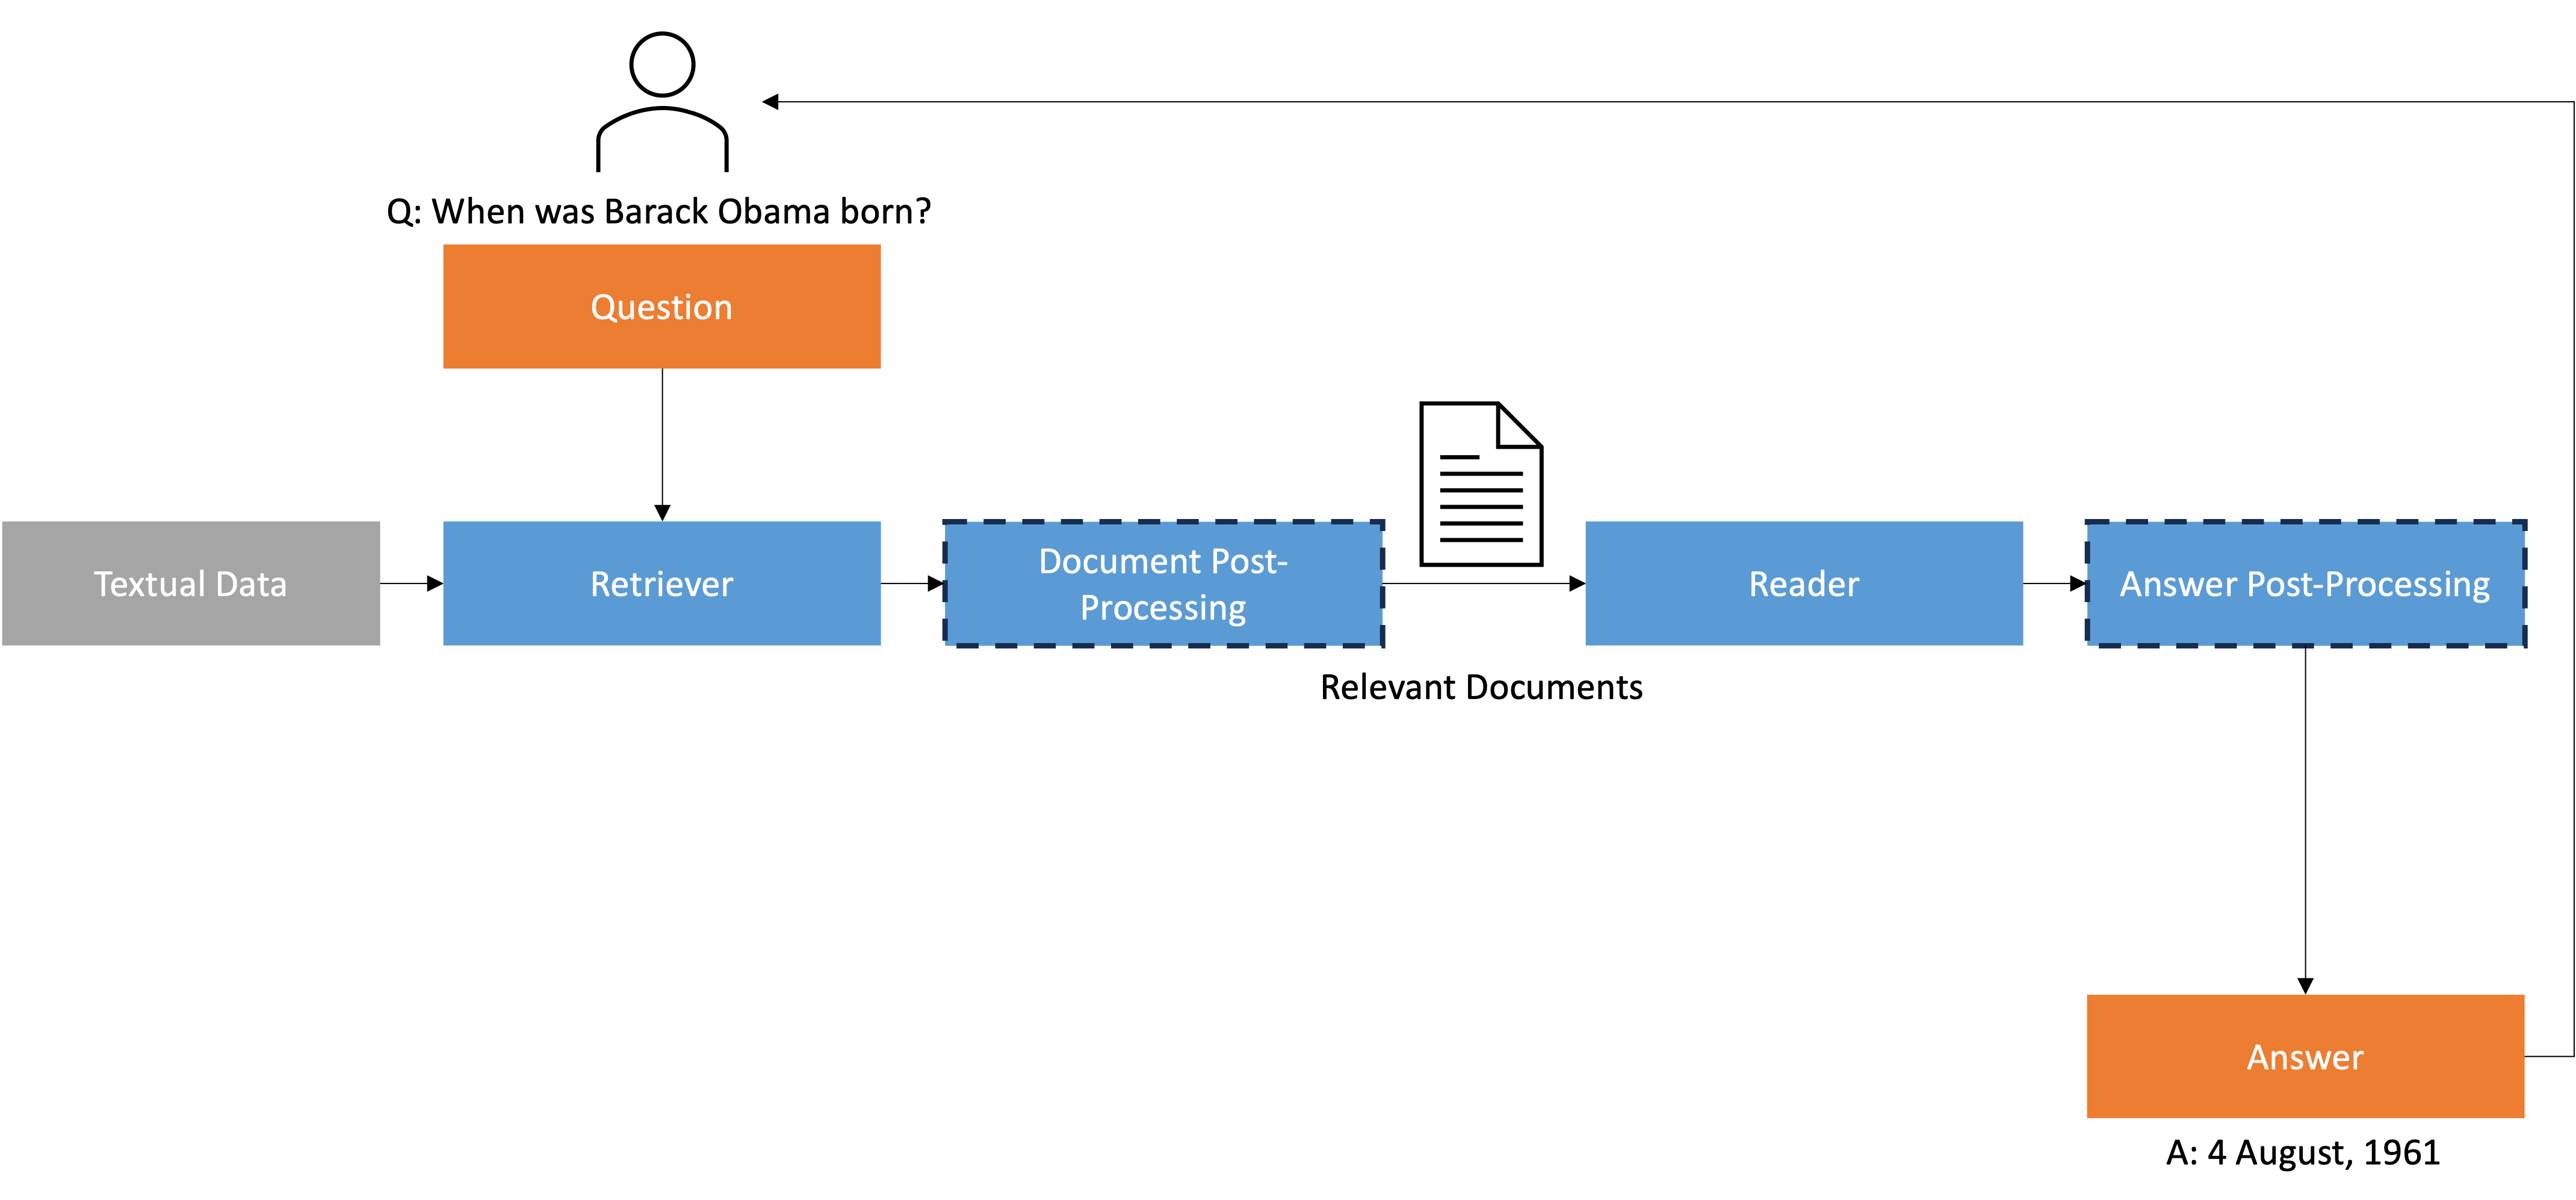
\includegraphics[width=\textwidth]{Grafiken/Retriever_Reader.png}
    \caption{Reader-Retriever-System Architecture for \gls{qa} by Zhu et. al. \cite{zhu_retrieving_2021}. The dashed lines indicate optional modules.}
    \label{fig:rr_architecture}
\end{figure}

Figure \ref{fig:rr_architecture} depicts the general architecture of a \textbf{Retriever-Reader-System}, as defined by Zhu et al. \cite{zhu_retrieving_2021}. This architecture serves as the foundational framework for \gls{ir}-Based \gls{qa} systems and was initially introduced by Harabagiu et al. \cite{harabagiu_open_domain_2003}. In this framework, all modules operate independently, can be trained separately, and are subject to independent evaluation.

The \textbf{Retriever} module's primary role is to retrieve relevant documents, passages, or other pertinent information from a knowledge source and rank them based on their relevance to answering the user's query. Subsequently, the \textbf{Reader} module extracts the answer from the retrieved documents and presents it to the user. This task bears a close resemblance to \gls{mrc}, with the key distinction that in \gls{ir}-Based \gls{qa}, the system must handle multiple documents and comprehend them to formulate a response, unlike classical \gls{mrc} tasks, which typically involve only one context document.

The \textbf{Document Post-Processor} module's role is to curate and refine the set of documents that will be forwarded as "Relevant Documents" to the subsequent stage, the Reader. Concurrently, the \textbf{Answer Post-Processor} assists the Reader in addressing complex questions for which the answer may not be found in a single document alone \cite{zhu_retrieving_2021,jurafsky_speech_2023}.

It's worth noting that some researchers include a \textbf{Question Analysis} module preceding the Retriever, which aims to preprocess the received question for more efficient query execution in the Retriever \cite{nassiri_transformer_2023}. However, for the purposes of this thesis, we adhere to Zhu et al.'s definition \cite{zhu_retrieving_2021}, where this functionality is considered part of the Retriever.

Conceptually, there are three distinct approaches to the Retriever itself: \textit{Sparse Retrieval, Dense Retrieval,} and \textit{Iterative Retrieval.} The specifics of these approaches will be thoroughly explored in Section \ref{subsec:qa_retrieval}.

Document Post-Processors can be categorized into \textit{Supervised Learning, Reinforcement Learning,} and \textit{Transfer Learning}-based approaches. A detailed discussion of these approaches is also provided in Section \ref{subsec:qa_retrieval}.

In Section \ref{subsec:qa_user_interaction}, we will delve into the finer details of Reader approaches and Answer Post-processing. Broadly speaking, there are two primary types of Readers: \textit{Extractive} and \textit{Generative} Readers. As for Answer Post-processing, it involves two key categories: \textit{Rule-based} and \textit{Learning-based} approaches.

There are also \textit{End-to-End} approaches that employ a single module to execute the entire \gls{qa} task. Excluding generative approaches, two common categories of such approaches are \textbf{Retriever-Reader} and \textbf{Retriever-only} models.

An End-to-End Retriever-Reader aims to train both the Retriever and Reader in a single backpropagation step, and in some cases, it introduces additional knowledge sources beyond the traditional \gls{ir} framework. An illustrative example is \gls{rag} \cite{lewis_retrieval-augmented_2021}. \gls{rag} consists of a pre-trained Generator with implicit knowledge encoded in its parameters and a pre-trained Retriever. For each question, the Retriever identifies the most relevant documents and generates a latent vector based on them. This latent vector, along with the original question, is fed into the Generator.

Another end-to-end approach, similar to \gls{rag}, is \gls{realm} \cite{guu_realm_2020}. While these previous two approaches extended the capabilities of pre-trained \gls{s2s} models, Nishida et al. pursued a different path by training a single \gls{nn} to perform both tasks simultaneously: \gls{ir} and \gls{mrc} \cite{nishida_retrieve-and-read_2018}.

It is noteworthy that all these end-to-end approaches have demonstrated competitive performance compared to state-of-the-art methods on specific \gls{qa} datasets.

An essential yet often underestimated question is: What defines textual data, and how should one preprocess formats such as PDFs to extract this textual content? While many datasets already comprise small contextual snippets, it's crucial not to overlook the entire process of extracting snippets from unstructured PDFs, for example. Approaches to tackle this challenge will be explored in detail in the upcomming Section \ref{subsec:qa_indexing}.

\subsection{Indexing Approaches}
\label{subsec:qa_indexing}

\subsection{Retrieval Approaches}
\label{subsec:qa_retrieval}

\subsection{Reader Approaches}
\label{subsec:qa_user_interaction}


\subsection{Limitations}
\label{subsec:qa_limitations}

\section{Conversational Question Answering}
\label{sec:cqa}

\section{Related Work}
\label{sec:related_work}